\section{Risultati}


\begin{frame}[fragile]{Risultati Intermedi}
Utilizzando il flag \verb|-v| o \verb|--verbose| vengono stampati \textbf{risultati intermedi}...
\begin{lstlisting}[style=statale, basicstyle=\tiny]
--- Checking host ---                                                                                                                                                                                                
Host is up                                                                                                                                                                                          
--- Checking ports ---                                                                                                                                                                                               
PORT       STATUS                                                                                                                                                                                                    
21         open                                                                                                                                                                                                      
22         open                                                                                                                                                                                                      
23         open                                                                                                                                                                                                      
--- Checking protocols and services ---                                                                                                                                                                              
PORT       PROTOCOL        SERVICE                                                                                                                                                                                   
21         FTP             (vsFTPd 2.3.4)                                                                                                                                                                            
22         SSH             SSH-2.0-OpenSSH_4.7p1 Debian-8ubuntu1                                                                                                                                                     
23         TELNET          undefined                                                                                                                                                                                
\end{lstlisting}

...e lo \textbf{stato attuale dell'esecuzione}
\begin{lstlisting}[style=statale, basicstyle=\tiny]
--- Checking protocols and services ---
Scanning 80 for FTP
\end{lstlisting}
\begin{lstlisting}[style=statale, basicstyle=\tiny]
--- Testing protocols and services ---  
Scanning 21 with FTP - (vsFTPd 2.3.4) using BACKDOOR COMMAND EXECUTION [1/1]
\end{lstlisting}
\end{frame}

%=======================================================================

\begin{frame}[fragile]{Risultati TXT}
    \begin{lstlisting}[style=statale, basicstyle=\tiny]
    ##### RESULTS FOR 192.168.100.175 #####

    PORT 	 PROTOCOL 	 SERVICE
    ----------------------------
    
    21         FTP             (vsFTPd 2.3.4)             
    |
    | --------------- VERSION CHECK ---------------
    |\___ THIS SERVICE VERSION IS VULNERABLE AND NEEDS TO BE UPDATED!
    |     reference:
    |     - CVE-2011-2523: https://www.cve.org/CVERecord?id=CVE-2011-2523
    |
    | --------------- VULNERABILITIES ---------------
    |\___ BACKDOOR COMMAND EXECUTION
    |     description: Allows users to leverage a backdoor to make a command execution.
    |     severity: high
    |
    | --------------- AUTHENTICATED VULNERABILITIES ---------------
    |\___ BOUNCE ATTACK
    |     description: If not correctly configured the PORT command can use the victim machine to request access to port indirectly. This can be used to scan hosts ports discretely.
    |     severity: medium
    \end{lstlisting}
\end{frame}

%=======================================================================

\begin{frame}[fragile]{Risultati JSON}
\begin{lstlisting}[style=statale, basicstyle=\tiny]
    "port": 21,
    "protocol": "FTP",
    "service": "(vsFTPd 2.3.4)",
    "unsafe_version": true,
    "unsafe_version_cve": [
        "https://www.cve.org/CVERecord?id=CVE-2011-2523"
    ],
    "vulnerabilities": [
        {
            "name": "BACKDOOR COMMAND EXECUTION",
            "service": "(vsFTPd 2.3.4)",
            "description": "Allows users to leverage a backdoor to make a command execution.",
            "severity": "high"
        }
    ],
    "auth_vulnerabilities": [
        {
            "name": "BOUNCE ATTACK",
            "service": "(vsFTPd 2.3.4)",
            "description": "If not correctly configured the PORT command can use the victim machine to request access to port indirectly. This can be used to scan hosts ports discretely.",
            "severity": "medium"
        }
    \end{lstlisting}
\end{frame}

\begin{frame}{Risultati HTML}
\begin{columns}
\begin{column}{0.5\textwidth}
    \begin{figure}
    \centering
    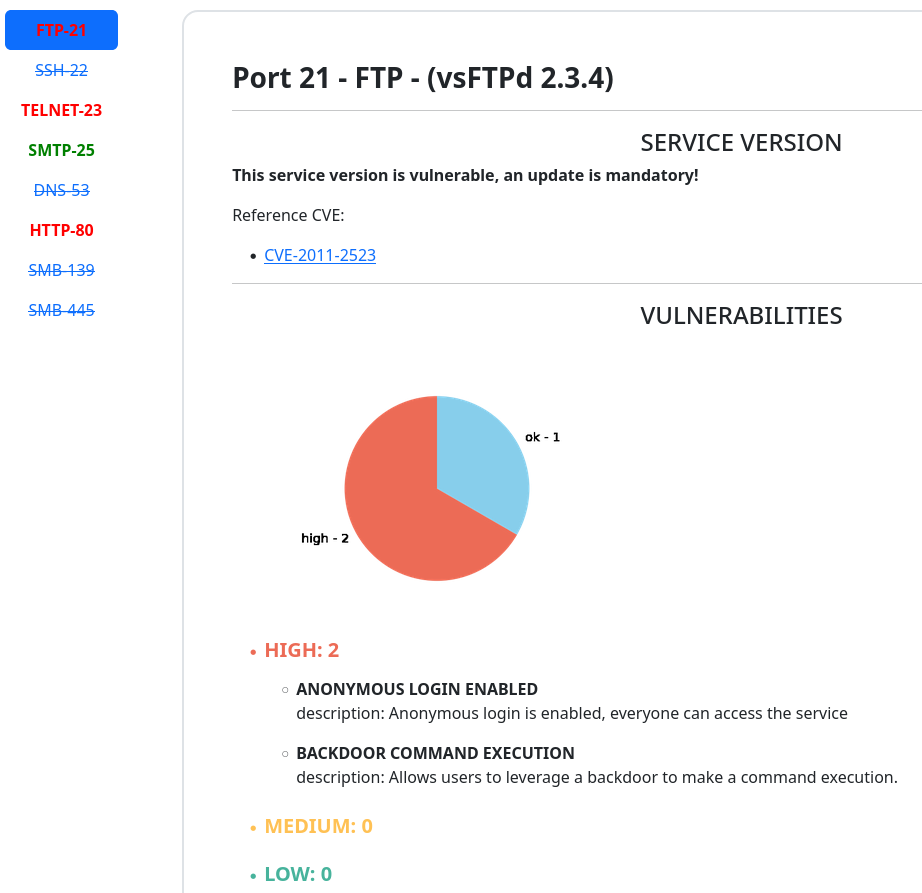
\includegraphics[width=6cm]{assets/mio/html_res1.png}
    \end{figure}
\end{column} 
\begin{column}{0.5\textwidth}
    \begin{figure}
    \centering
    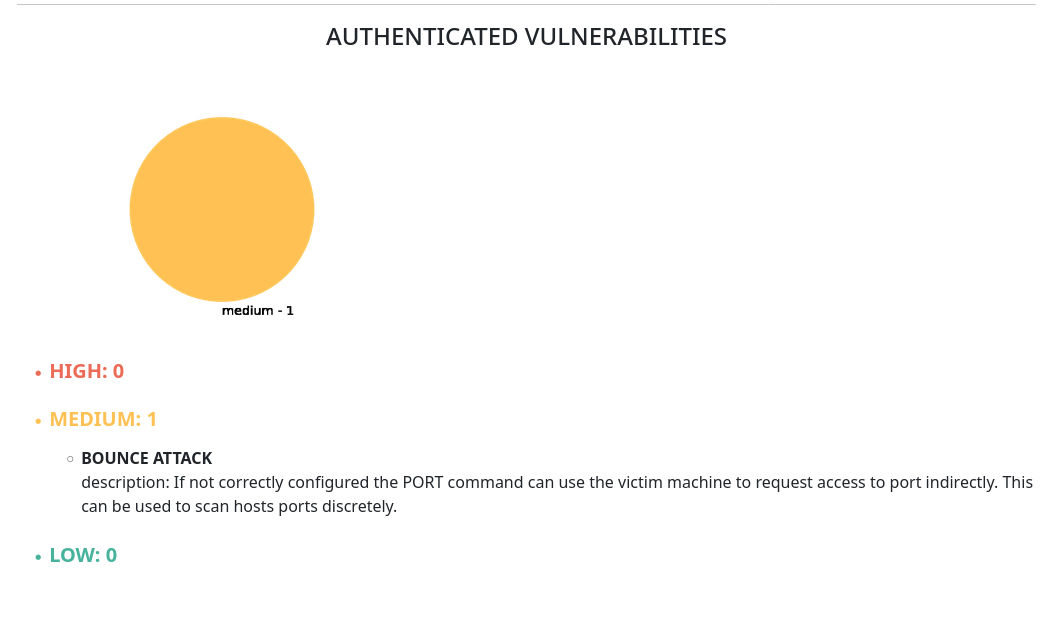
\includegraphics[width=7cm]{assets/mio/html_results2.png}
    \end{figure}
\end{column} 
\end{columns}
\end{frame}